\documentclass{beamer}
\usepackage{relsize}
\usepackage{color}

\usepackage{listings}
\usetheme{CambridgeUS}
%\usepackage{beamerthemesplit} % new
\usepackage{enumitem}
\usepackage{amsmath}                    % See geometry.pdf to learn the layout options.
\usepackage{amsthm}                   % See geometry.pdf to learn the layout options. There
\usepackage{amssymb}                    % See geometry.pdf to learn the layout options.
\usepackage[utf8]{inputenc}
\usepackage{graphicx}
\usepackage[english,bulgarian]{babel}
\usepackage{tikz}
\usepackage{forest}
\usetikzlibrary{positioning,fit,calc}


\lstset{language=C++,
                basicstyle=\ttfamily,
                keywordstyle=\color{blue}\ttfamily,
                stringstyle=\color{black}\ttfamily,
                commentstyle=\color{blue}\ttfamily,
                morecomment=[l][\color{magenta}]{\#}
}

\newtheorem{mydef}{Дефиниция}[section]
\newtheorem{lem}{Лема}[section]
\newtheorem{thm}{Твърдение}[section]

\DeclareMathOperator{\restrict}{\upharpoonright}

\setitemize{label=\usebeamerfont*{itemize item}%
  \usebeamercolor[fg]{itemize item}
  \usebeamertemplate{itemize item}}

\setbeamercovered{transparent}

\tikzset{
block/.style = {draw, fill=white, rectangle,align = center},
entry/.style = {draw, fill=black, circle, radius=3em},
condition/.style = {draw, fill=white, diamond, align = center,node distance=3cm},
fork/.style = {draw, fill=black, circle,inner sep=1pt},
lnode/.style={rectangle split, rectangle split parts=3,draw, rectangle split horizontal},
treenode/.style = {align=center, inner sep=0pt, text centered, circle, font=\sffamily\bfseries, draw=white, fill=white, text width=1.5em}
}



\begin{document}
\title[Обектно ориентирано програмиране]{Наследяване и композиция. Visitor Pattern.}
\author{Калин Георгиев}
\frame{\titlepage}

\section{Наследяване и композиция}

\begin{frame}[fragile]
\frametitle{Примерен казус}
%\vspace{-60px}
\begin{center}
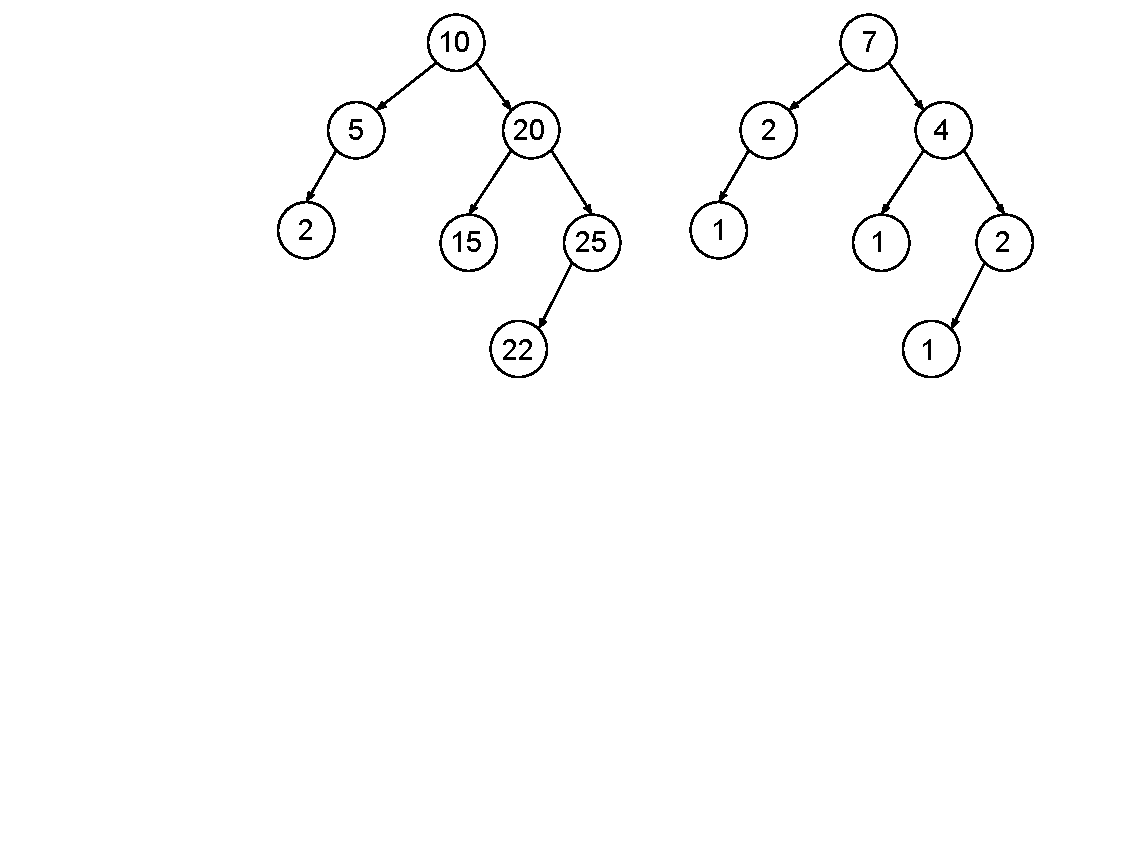
\includegraphics[width=10.0cm]{images/tree1}
\end{center}
\end{frame}


\begin{frame}[fragile]
\frametitle{Структура на обекта}

\begin{tikzpicture}[auto, node distance=1cm,>=latex]
  
  \node  [] (ttl){Drawing};
  \node  [below of=ttl, rectangle split, rectangle split parts=3,draw, rectangle split horizontal] (arr1) 
      {\nodepart[text width=1.5cm]{one}Rectangle
       \nodepart[text width=1.5cm]{two}Circle
       \nodepart[text width=1.5cm]{three}Group};

       \node[fit=(arr1)(ttl), draw] (obj1) {};

  \node  [below right of = obj1, node distance = 3.5cm] (ttl2){Drawing};
  \node  [below of=ttl2, rectangle split, rectangle split parts=2,draw, rectangle split horizontal] (arr2) 
      {\nodepart[text width=1.5cm]{one}Rectangle
      \nodepart[text width=1.5cm]{two}Group};

      \node[fit=(arr2)(ttl2), draw] (obj2) {};
  \draw[->]  (arr1.three)-- (obj2);   
\end{tikzpicture}


\end{frame}
    

\begin{frame}
  \centerline{Visitor Pattern!}
\end{frame}
  

\begin{frame}[fragile]
  \frametitle{Конкретни елементи $\times$ конкретни операции. Double Dispatch.}

\begin{tabular}{c | c | c}
             & Serialize & Draw \\\hline
  Rectangle  & Rectangle::serialize & rectangle::draw \\\hline
  Circle  & Circle::serialize & Circle::draw \\\hline
  Triangle  & Triangle::serialize & Triangle::draw \\\hline
  Group  & Group::serialize & Group::draw 
\end{tabular}

\end{frame}
  



\begin{frame}[fragile]
  \frametitle{Visitor Pattern}
  
  \begin{centering}
  \relscale{0.6}
  \begin{tikzpicture}[auto, node distance=1.2cm,>=latex]
    
    \node  [] (title1){Rectangle};
    \node  [block,align=left,below of=title1,draw] (proc1) 
      {virtual Process\_ME(visitor)\\-Process\_Rectangle(this)};
    \node[fit=(title1)(proc1), draw] (rect) {};
  
    \node  [below of = proc1] (title2){Cicrcle};
    \node  [block,align=left,below of=title2,draw] (proc2) 
      {virtual Process\_ME(visitor)\\-Process\_Circle(this)};
    \node  [fit=(title2)(proc2), draw] (circ) {};

    \node  [below of = proc2] (title3){Group};
    \node  [block,align=left,below of=title3,draw] (proc3) 
    {virtual Process\_ME(visitor)\\-Process\_Group(this)};
    \node  [fit=(title3)(proc3), draw] (group) {};

    \node  [right of = proc1, node distance = 4cm] (title4){Serializer};
    \node  [below of=title4,draw] (proc4) {Process\_Rectangle};
    \node  [below of=proc4,draw] (proc5) {Process\_Circle};
    \node  [below of=proc5,draw] (proc6) {Process\_Group};
    \node  [fit=(title4)(proc4)(proc5)(proc6), draw] (ser1) {};

    \draw[->]  (proc1)-- (proc4);   
    \draw[->]  (proc2)-- (proc5);   
    \draw[->]  (proc3)-- (proc6);   

    %\draw[->]  (proc6.east) -| node[right of = proc6, distance=5cm]{a} (proc4.east);   
    \draw[->] (proc6.east) -| ([xshift=1.5cm,yshift=0cm]proc5.east) |- (proc4.east);    
    \draw[->] (proc6.east) -| ([xshift=1.5cm,yshift=0cm]proc5.east) |- (proc5.east);    
    %\draw[->]  (proc6)-- (proc5);   

    \node  [block,align=left,left of=proc2,draw, node distance = 4cm] (call) 
    {figure->process\_me(serializer)};

    \draw[->]  (call)-- (rect);   
    \draw[->]  (call)-- (circ);   
    \draw[->]  (call)-- (group);   


  \end{tikzpicture}
\end{centering}
  
  
  \end{frame}
  






\begin{frame}
\centerline{Благодаря ви за вниманието!}
\end{frame}

\end{document}



\begin{columns}[t]
  \begin{column}{0.55\textwidth}

  \end{column}
  \begin{column}{0.45\textwidth}

  \end{column}
\end{columns}
